% Document notes
% Interestingly, in Figure 1, need to draw the node first, then fill it in order to still have a visible label on the node. See the circle node (tikzstyle) specifications.
% Forget what \raggedbottom does, so deleted it. Uhhhhhhh... Actually without it the spacing is weird between sections. Put it back in.
\documentclass [12pt, letterpaper, twoside]{article}
\usepackage[utf8]{inputenc}
\usepackage [left=1.0in, right=1.0in, top=1.0in, bottom=1.0in]{geometry}
% For updated time
\usepackage{datetime}
% For drawing pictures
\usepackage{tikz}
% For equations
\usepackage{amsmath}
% To make tables
\usepackage{tabu}
% For multiple rows in table slot
\usepackage{multirow}
% To add captions
\usepackage{caption}
% To make scatter plots
\usepackage{pgfplotstable}
% Reference local figures and tables
\usepackage{hyperref}

\usetikzlibrary{positioning}

\pgfplotsset{compat=1.16}
\raggedbottom
\begin{document}
\begin{titlepage}
\begin{center}
College of Science: Physics Department \\
\vspace{0.1cm}
Illinois Institute of Technology\\
\vspace{0.1cm}
General Physics II: Electromagnetism (PHYS 221-01)\\
\vspace*{\fill}
\begingroup
\Large
\textbf{Coulomb's Law}
\vspace{0.35cm}

\normalsize
Lab 1
\vspace{1.5cm}
\endgroup
\vspace*{\fill}
\end{center}

\vspace*{\fill}
\begin{flushright}
\footnotesize
Emily Pang, Lavanya Roy (lab partner) \\
Date of experiment: 29 Jan 2020 \\
Due date: 5 Feb 2020 \\
Lab section L06 \\
TA: Will Limestall \\
Updated \usdate\today~(\currenttime)
\end{flushright}
\end{titlepage}

\subsection*{STATEMENT OF OBJECTIVE}
The objective of this lab was to examine the relationship between charged masses and the distance between charges using Coulomb's Law.

\subsection*{THEORY}
When two or more charged particles are within some distance \(r\), the force exerted on the particles by each other can be modeled using Coulomb's Law, as shown below:
\begin{equation} \label{eq:1}
    F = k\dfrac{q_{1}q_{2}}{r^2} \\
\end{equation}
where \(k\) is a constant measured at 9.0 \(\times 10^9 \tfrac{\text{ N}\cdot\text{m}^2}{\text{C}^2}\) and the force is measured in Newtons. Additionally, all masses exert a gravitational force on other masses, as shown by the Law of Universal Gravitation:
\begin{equation}
  \begin{split}
    F_{\text{univ. grav.}} &= G\dfrac{m_{1}m_{2}}{r^2} \\
  \end{split}
\end{equation}
where \(G\) is a constant equal to \(6.67\times{10^{-11}}\tfrac{\text{m}^2}{\text{kg}\cdot{\text{s}^2}}\), \(m_{1}\) and \(m_{2}\) represent the two masses, and \(r\) is the distance between the centers of the masses. Lastly, it is known that all masses on Earth are under the influence of gravity (including Earth). The force of gravity on a mass on Earth is represented by:
\begin{equation}
  \begin{split}
    F_{\text{gravity}} &= mg \\
  \end{split}
\end{equation}
where \(m\) is the mass of the object and \(g\) is the gravity constant on Earth, 9.8 \(\tfrac{\text{m}}{\text{s}^2}\). With this information, it is proposed that two equal charges can be calculated with Coulomb's Law using the already proven ideas of gravity on Earth.

\subsection*{EQUIPMENT}
  \noindent
  \begin{itemize}
    \itemsep0em
    \item{two pith balls}
    \item{one simple electroscope}
    \item{mirror ruler}
    \item{two strings}
    \item{one acrylic rod}
    \item{one nylon rod}
    \item{one rayon rod}
    \item{one rubber rod}
    \item{one vinyl rod}
    \item{silk}
    \item{wool}
    \item{plastic bag sheet}
    \item{hair}
    \item{mystery fur}
  \end{itemize}

\subsection*{PROCEDURE}
First, the electroscope should be set up as shown in Figure ~\ref{fig:1}, with both pith balls attached to the electroscope with an equal length of string. \(r\) will be equal to zero initially as the balls are not charged. Each of the rod-material combinations will be rubbed together to statically charge the rods. Figure 2 from the IIT lab manual (IIT, 2) shows the material and rod affinities for receiving or giving electrons.

After charging a rod, it will be dragged across the metal support of the electroscope, charging the pith balls. The distance between the pith balls will then be measured using the mirror ruler. Care should be taken to not discharge the pith balls by touching them. This procedure will be repeated for each of the rod-material combinations and \(r\) will be recorded.

In order to completely use Coulomb's Law, it needs to be used alongside a known equation. In this experiment, Newton's Law of Universal Gravitation will be used. Thus, the length of the string will also need to be recorded to calculate the gravitational force. The mass of the pith balls is given in the lab manual.

\begin{figure}
  \begin{center}
    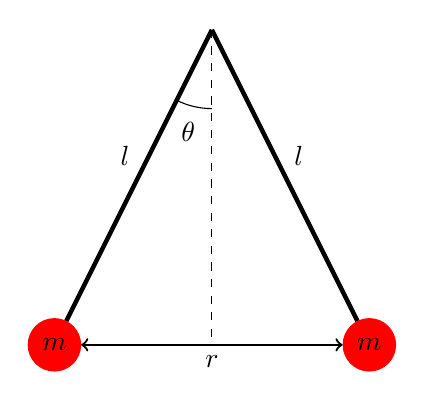
\begin{tikzpicture}
      \tikzstyle{ball}=[circle,draw,minimum size=1.0,draw=red,fill=red]
      \tikzstyle{string}=[ultra thick,draw]
      % Coordinate to connect strings
      \coordinate (stand) at (2,4) {};
      % Pith balls
      \node (ball1) at (0,0) [ball] {\(m\)};
      \node (ball2) at (4,0) [ball] {\(m\)};
      % Draw lines to balls
      \draw (stand) -- node[above left] {\(l\)} ++(ball1) [string];
      \draw (stand) -- node[above right] {\(l\)} ++(ball2) [string];
      % r line
      \draw [<->,thick] (ball1) -- node[below] {\(r\)} ++(ball2);
      % Dashed line
      \draw [dashed] (stand) -- (2,0);
      % Theta angle
      % Wish to replace with a circle so don't have to calculate where to place arc
      \draw (1.553,3.106) arc [radius=1.0cm, start angle=243.4, end angle=270];
      \node at (1.7,2.7) {\(\theta\)};
    \end{tikzpicture}
    \caption{Pith balls on a string of length \(l\) with mass \(m\) and a distance \(r\) from each other.}
    \label{fig:1}
  \end{center}
\end{figure}

\subsection*{DATA}
Each combination of rod and material was used to charge the rod and apply it to the pith balls. The distance was then recorded for three trials. These trials are shown in Table ~\ref{tab:1}. Tables ~\ref{tab:2} and ~\ref{tab:3} show the charge force, \(F_{\text{charge}}\), and charge magnitude, \(|q|\), for each rod/material pair. The mass of each pith ball was 0.04 grams per the lab manual (IIT, 3). The length of the string was not measured, but a value of 9.3 cm was used.

\begin{table}
  \centering
  \begin{tabular}{| c | c | r | r | r | r |}
    \hline\hline
    & & \multicolumn{4}{ c |}{Rods} \\
    \hline
    & & Rubber & Nylon & Acrylic & Vinyl \\
    \hline
    \multirow{16}{*}{Material} & \multirow{3}{*}{Silk} & 0.0570 & 0.0080 & 0.0740 & 0.0250 \\
    & & 0.0550 & 0.0050 & 0.0660 & 0.0570 \\ 
    & & 0.0565 & 0.0070 & 0.0520 & 0.0660 \\
    \cline{2-6}
    & Average & 0.0562 & 0.00667 & 0.064 & 0.0493 \\ %66667 (LDR) %6667 (LDR) % %33333 (LDR)
    \cline{2-6}
    & \multirow{3}{*}{Plastic} & 0.0430 & 0.0070 & 0.0780 & 0.0640 \\
    & & 0.0300 & 0.0110 & 0.0640 & 0.0670 \\
    & & 0.0360 & 0.0090 & 0.0300 & 0.0640 \\
    \cline{2-6}
    & Average & 0.0363 & 0.009 & 0.0573 & 0.0650 \\ %33333 (LDR) % %33333 %
    \cline{2-6}
    & \multirow{3}{*}{Hair} & 0.0570 & 0.0620 & 0.0450 & 0.0710 \\
    & & 0.0600 & 0.0710 & 0.0650 & 0.0610 \\
    & & 0.0650 & 0.0660 & 0.0630 & 0.0660 \\
    \cline{2-6}
    & Average & 0.0607 & 0.0663 & 0.0577 & 0.0660 \\ %66667 (LDR) %33333 %66667 (LDR) %
    \cline{2-6}
    & \multirow{3}{*}{Wool} & 0.0480 & 0.0170 & 0.0340 & 0.0700 \\
    & & 0.0240 & 0.0060 & 0.0300 & 0.0730 \\
    & & 0.0300 & 0.0070 & 0.0560 & 0.0750 \\
    \cline{2-6}
    & Average & 0.0340 & 0.0100 & 0.0400 & 0.0727 \\ % % % %66667 (LDR)
    \cline{2-6}
    \hline\hline
  \end{tabular} \\
  \caption{Distance between pith balls in meters between different rods and materials}
  \label{tab:1}
\end{table}

\begin{table}
  \centering
  \begin{tabular}{| c | c | c | c | c | c | c | c | c | c |}
    \hline\hline
    & & \multicolumn{4}{ c |}{Rods} \\
    \hline
    & & \multicolumn{2}{ c |}{Rubber} & \multicolumn{2}{ c |}{Nylon} \\
    \hline
    & & \(F_{\text{charge}}\) (N) & \(|q|\) (C) & \(F_{\text{charge}}\) (N) & \(|q|\) (C) \\ 
    \hline
    \multirow{4}{*}{Material} & Silk & 0.000124 & 6.60 \(\times 10^{-9}\) & 0.0000141 & 2.63 \(\times 10^{-10}\) \\ %169358 %727543 (LDR) %592135 (LDR) %492357 %65347 (LDR) %568429 (LDR) %83345 (LDR) %002727
    \cline{2-6}
    & Plastic & 0.0000781 & 3.38 \(\times 10^{-9}\) & 0.0000190 & 4.13 \(\times 10^{-10}\) \\ %776033 (LDR) %413143 %899857 (LDR) %412471 %016292 %107479 %207576 %470485
    \cline{2-6}
    & Hair & 0.000135 & 7.44 \(\times 10^{-9}\) & 0.000150 & 8.55 \(\times 10^{-9}\) \\ %253239 %708455 (LDR) %638717 (LDR) %327732 %833041 (LDR) %26647 %778135 (LDR) %578913 (LDR)
    \cline{2-6}
    & Wool & 0.0000729 & 3.06 \(\times 10^{-9}\) & 0.0000211 & 4.84 \(\times 10^{-10}\) \\ %839413 (LDR) %966295 (LDR) %057941 %261111 %207909 %738668 (LDR) %368938 %984447 (LDR)
    \cline{2-6}
    \hline\hline
  \end{tabular} \\
  \caption{Force of charge and charge values for rubber and nylon}
  \label{tab:2}
\end{table}

\begin{table}
  \centering
  \begin{tabular}{| c | c | c | c | c | c |}
    \hline\hline
    & & \multicolumn{4}{ c |}{Rods} \\
    \hline
    & & \multicolumn{2}{ c |}{Acrylic} & \multicolumn{2}{ c |}{Vinyl} \\
    \hline
    & & \(F_{\text{charge}}\) (N) & \(|q|\) (C) & \(F_{\text{charge}}\) (N) & \(|q|\) (C) \\ 
    \hline
    \multirow{4}{*}{Material} & Silk & 0.000144 & 8.09 \(\times10^{-9}\) & 0.000108 & 5.40 \(\times 10^{-9}\) \\
    \cline{2-6}
    & Plastic & 0.000127 & 6.81 \(\times10^{-9}\) & 0.000146 & 8.28 \(\times 10^{-9}\) \\
    \cline{2-6}
    & Hair & 0.000128 & 6.87 \(\times10^{-9}\) & 0.000149 & 8.49 \(\times 10^{-9}\) \\
    \cline{2-6}
    & Wool & 0.0000863 & 3.92 \(\times10^{-9}\) & 0.000166 & 9.88 \(\times10^{-9}\) \\
    \hline\hline
  \end{tabular}
  \caption{Force of charge and charge values for acrylic and vinyl}
  \label{tab:3}
\end{table}

\subsection*{ANALYSIS OF DATA}
Figures ~\ref{fig:2}, ~\ref{fig:3}, ~\ref{fig:4}, and ~\ref{fig:5} show the distance between the pith balls depending on the rod and material combination. Equation 9 from Supplementary Question 1 can be used to measure the force from Coulomb's Law. Figure ~\ref{fig:6} shows the force of the two charges using Equation 9 and the distance between the charges, while Figure ~\ref{fig:7} is a direct representation of Equation 13 and explores the distance between charges and the charge values themselves.

\begin{figure}
  \centering
  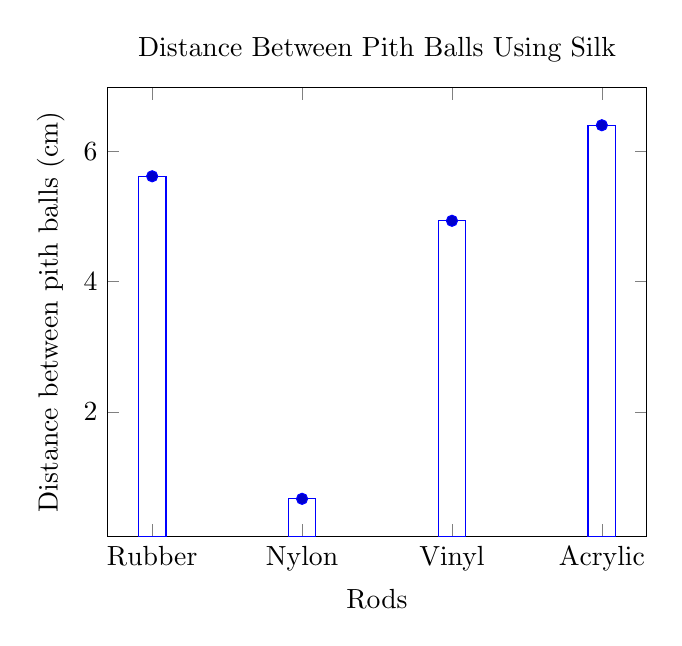
\begin{tikzpicture}
    \begin{axis}[
      title = {Distance Between Pith Balls Using Silk},
      symbolic x coords = {Rubber, Nylon, Vinyl, Acrylic},
      xtick = data,
      nodes near coords align={vertical},
      xlabel = {Rods},
      ylabel = {Distance between pith balls (cm)},
    ]
    \addplot+[ybar] plot coordinates
      {(Rubber,5.6166667) (Nylon, 0.6666667) (Vinyl,4.9333333) (Acrylic,6.4)};
    \end{axis}
  \end{tikzpicture}
  \caption{}
  \label{fig:2}
\end{figure}

\begin{figure}
  \centering
  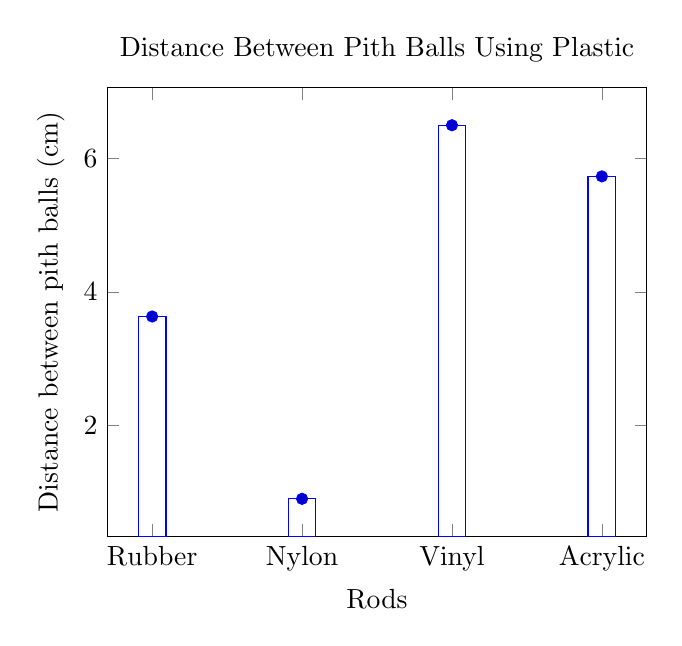
\begin{tikzpicture}
    \begin{axis}[
      title = {Distance Between Pith Balls Using Plastic},
      symbolic x coords = {Rubber, Nylon, Vinyl, Acrylic},
      xtick = data,
      nodes near coords align={vertical},
      xlabel = {Rods},
      ylabel = {Distance between pith balls (cm)},
    ]
    \addplot+[ybar] plot coordinates
        {(Rubber,3.6333333) (Nylon,0.9) (Vinyl,6.5) (Acrylic,5.7333333)};
    \end{axis}
  \end{tikzpicture}
  \caption{}
  \label{fig:3}
\end{figure}

\begin{figure}
  \centering
  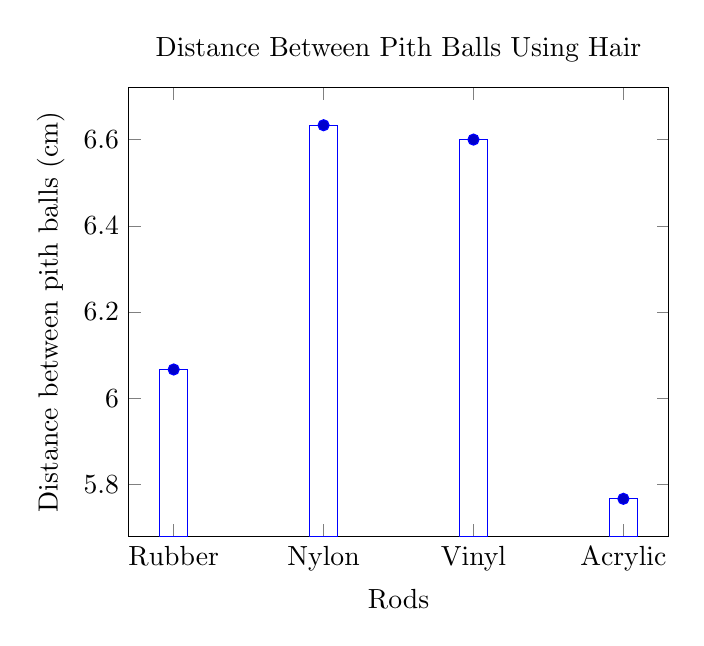
\begin{tikzpicture}
    \begin{axis}[
      title = {Distance Between Pith Balls Using Hair},
      symbolic x coords = {Rubber, Nylon, Vinyl, Acrylic},
      xtick = data,
      nodes near coords align={vertical},
      xlabel = {Rods},
      ylabel = {Distance between pith balls (cm)},
    ]
    \addplot+[ybar] plot coordinates
        {(Rubber,6.0666667) (Nylon,6.6333333) (Vinyl,6.6) (Acrylic,5.7666667)};
    \end{axis}
  \end{tikzpicture}
  \caption{}
  \label{fig:4}
\end{figure}

\begin{figure}
  \centering
  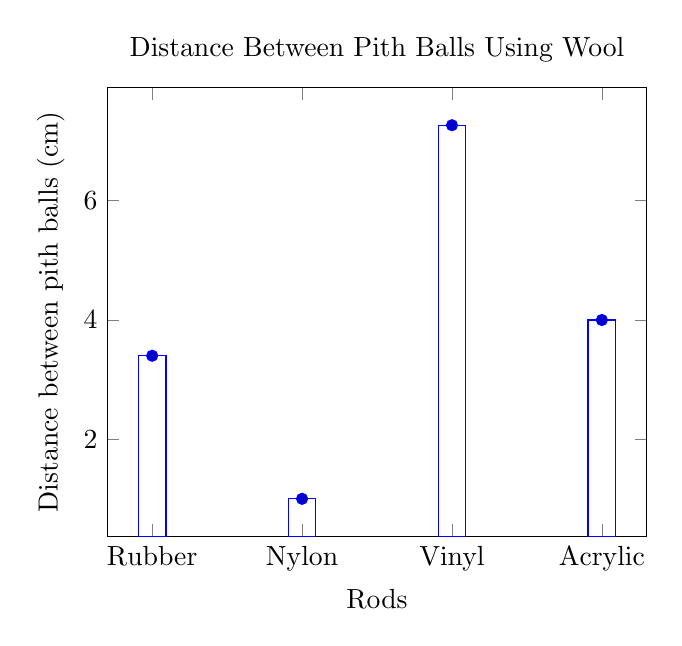
\begin{tikzpicture}
    \begin{axis}[
      title = {Distance Between Pith Balls Using Wool},
      symbolic x coords = {Rubber, Nylon, Vinyl, Acrylic},
      xtick = data,
      nodes near coords align={vertical},
      xlabel = {Rods},
      ylabel = {Distance between pith balls (cm)},
    ]
    \addplot+[ybar] plot coordinates
        {(Rubber,3.4) (Nylon,1) (Vinyl,7.2666667) (Acrylic,4)};
    \end{axis}
  \end{tikzpicture}
  \caption{}
  \label{fig:5}
\end{figure}

\pgfplotstableread{
X Y
5.6166667 124.169358 
0.6666667 14.0592135
6.4       143.65347
4.9333333 107.83345
3.6333333 78.0776033
0.9       18.9899857
5.7333333 127.016292
6.5       146.207576
6.0666667 135.253239
6.6333333 149.638717
5.7666667 127.833041
6.6       148.778135
3.4       72.8839413
1.0       21.1057941
4.0       86.3207909
7.2666667 166.368938
}\distanceAndForce

\begin{figure}
  \centering
  \begin{tikzpicture}
    \begin{axis}[
      title = {Distance Between Charges and Force of Charge},
      xlabel = {\(r\) (cm)},
      ylabel = {\(F_{\text{charge}}\) (\(\mu\)N)},
      ]
      \addplot [only marks, mark = *] table {\distanceAndForce};
      \addplot [thick, red] table[
        y={create col/linear regression={y=Y}}
      ]
      {\distanceAndForce};
    \end{axis}
  \end{tikzpicture}
  \caption{}
  \label{fig:6}
\end{figure}

\pgfplotstableread{
X Y
5.6166667 6.59727543
0.6666667 0.263492357
6.4       8.08568429
4.9333333 5.40002727

3.6333333 3.38413143
0.9       0.413412471
5.7333333 6.81107479
6.5       8.28470485

6.0666667 7.43708455
6.6333333 0.484261111
5.7666667 3.91738668
6.6       9.87984447

3.4       3.05966295
1.0       0.484261111
4.0       3.91738668
7.2666667 9.87984447
}\distanceAndCharge

\begin{figure}
  \centering
  \begin{tikzpicture}
    \begin{axis}[
      title = {Distance Between Charges and Charge Values},
      xlabel = {\(r\) (cm)},
      ylabel = {\(q\) (nC)},
      ]
      \addplot [only marks, mark = *] table {\distanceAndCharge};
      \addplot [thick, red] table[
        y={create col/linear regression={y=Y}}
      ]
      {\distanceAndCharge};
    \end{axis}
  \end{tikzpicture}
  \caption{}
  \label{fig:7}
\end{figure}

\subsection*{DISCUSSION OF RESULTS}
Figures 2 through 5 can be compared to what was expected for each rod/material combination. For instance, in Figure ~\ref{fig:2}, it was expected that the acrylic rod would show the greatest distance between pith balls followed by vinyl, with nylon and rubber being equal. However, the results showed that while acrylic discharged the most, nylon and rubber did not behave as expected.

For plastic, it was expected that acrylic would show the greatest distance, followed by nylon, vinyl, and then rubber. The lowest, as shown in Figure ~\ref{fig:3}, was nylon, which does not match expectations.

For hair, the expectation was for vinyl to discharge the greatest, followed by rubber, and equally, acrylic and nylon. However, nylon again disrupts expectations by having the greatest distance between the pith balls. Acrylic and rubber seem to follow expectations.

And lastly, for wool, vinyl was expected to show the greatest distance, followed by rubber, acrylic, and nylon. Figure ~\ref{fig:5} shows that these expectations were mostly met, with acrylic slightly exceeding the distance expected.

\subsection*{FURTHER STUDY}
The lab manual states that there are five materials to test (IIT, 3) and five rods to charge the pith balls with. The materials and rods presented at the lab station lacked both a mystery fur and a rayon rod, resulting in this experiment consisting of 16 rod/material combinations. Thus, if this experiment were to be repeated, the materials needed (see Equipment) should be thoroughly checked. Since this experiment did not contain the full list, it is less rigorous than had it been executed in full.

Additionally, the value for the length of the string was not recorded during the experiment. The value implemented in this lab report was obtained from another experiment, and as such, all representative material (tables and graphs) cannot fully model the actual experiment.

\subsection*{SUPPLEMENTARY QUESTIONS}
\begin{enumerate}
  \item{Using the free-body diagrams of Figure 3, derive an expression for the charge in terms of the pith ball mass \emph{m}, and the separation distance \(r\).}

    \begin{figure}
      \centering
      \begin{tikzpicture}
        \tikzstyle{ball}=[rectangle,draw,minimum size=1.5cm]
          \node (ball) at (0,0) [ball] {Ball};
          \node (GForce) at (0,-1.75) {\(F_{\text{gravity}}\)};
          \node (TForce) at (1,1.75) {\(F_{\text{tension}}\)};
          \node (CForce) at (-1.75,0) {\(F_{\text{charge}}\)};
          \draw [->] (ball) -- (GForce);
          \draw [->] (ball) -- (TForce);
          \draw [->] (ball) -- (CForce);
      \end{tikzpicture}
      \caption{FBD of Pith Ball}
      \label{fig:8}
    \end{figure}
    We know Coulomb's Law from Equation ~\ref{eq:1}. The gravitational force for the pith balls is equal to the product of the mass and Earth's gravity constant. Using this information and the fact that the pith balls are not moving, the following is derived:
    \begin{equation*}
      \begin{split}
        F_{\text{charge}} &= F_{\text{tension}}\sin{\theta} \\
      \end{split}
    \end{equation*}

    \noindent
    Additionally:
    \begin{equation}
      \begin{split}
        F_{\text{gravity}} &= F_{\text{tension}}\cos{\theta} \\
        m_{\text{ball}}g &= F_{\text{tension}}\cos{\theta} \\
      \end{split}
    \end{equation}

    \noindent
    where \(\theta\) is the angle between the string and the vertical. The tension force can be solved for using the above Equation set 4:
    \begin{equation}
      \begin{split}
        F_{\text{tension}} &= \dfrac{F_{\text{charge}}}{\sin{\theta}} \\
      \end{split}
    \end{equation}

    \noindent
    Likewise, Equation set 5 can be used to solve for the tension force:
    \begin{equation}
      \begin{split}
        F_{\text{tension}} &= \dfrac{m_{\text{ball}}g}{\cos{\theta}}
      \end{split}
    \end{equation}

    \noindent
    Thus, since \(F_{\text{tension}}\) is solved for in Equation set 6 and 7, they can be combined:
    \begin{equation}
      \begin{split}
        \dfrac{F_{\text{charge}}}{\sin{\theta}} &= \dfrac{m_{\text{ball}}g}{\cos{\theta}} \\
      \end{split}
    \end{equation}

    \noindent
    To find \(F_{\text{charge}}\) in this experiment, \(F_{\text{charge}}\) can be solved for:
    \begin{equation}
      \begin{split} 
        F_{\text{charge}} &= m_{\text{ball}}g\tan{\theta} \\
      \end{split}
    \end{equation}

    \noindent
    To find \(q_{1}\) and \(q_{2}\), it must be known that these charges are equal, since they were equally charged by the rods. Thus, by substituting in Coulomb's Law (Equation 1), the charge on a pith ball, \(q\), can be solved for:
    \begin{equation}
      \begin{split}
        k\dfrac{q_{1}q_{2}}{r^2} &= m_{\text{ball}}g\tan{\theta} \\
        k\dfrac{q^2}{r^2} &= m_{\text{ball}}g\tan{\theta} \\
        q &= \sqrt{\dfrac{r^{2}m_{\text{ball}}g\tan{\theta}}{k}} \\
      \end{split}
    \end{equation}

    \noindent
    However, \(\theta\) was not measured. Using trig:

    \begin{equation}
      \begin{split}
        \theta &= \sin^{-1}\left(\dfrac{r}{2l}\right) \\
      \end{split}
    \end{equation}

    \noindent
    where \(l\) is the length of the string. Finally, Equation 10 can be combined with Equation 11 to calculate the charge force and charge on a pith ball using the mass of the ball and the length of the string. Below is how to calculate the charge force:

    \begin{equation}
      \begin{split}
        F_{\text{charge}} &= m_{\text{ball}}g\tan{\theta} \\
        F_{\text{charge}} &= m_{\text{ball}}g\tan\left({\sin^{-1}\left(\dfrac{r}{2l}\right)}\right) \\
        F_{\text{charge}} &= m_{\text{ball}}g\left(\dfrac{r}{\sqrt{4l^2-r^2}}\right) \\
      \end{split}
    \end{equation}

    \noindent
    Below is how to calculate the charge on a single pith ball:
    \begin{equation*}
      \begin{split}
        q &= \sqrt{\dfrac{r^{2}m_{\text{ball}}g\tan{\theta}}{k}} \\
        q &= \sqrt{\dfrac{r^{2}m_{\text{ball}}g\tan{\left(\sin^{-1}\left(\dfrac{r}{2l}\right)\right)}}{k}} \\
        q &= \sqrt{\dfrac{r^{2}m_{\text{ball}}g\left(\dfrac{r}{\sqrt{4l^2-r^2}}\right)}{k}} \\
        q &= \sqrt{\dfrac{r^{3}m_{\text{ball}}g}{k\sqrt{4l^2-r^2}}} \\
      \end{split}
    \end{equation*}

  \item{Calculate the charge on the pith balls for each rod/soft material combination. How many millions or billions of electrons reside on each pith ball?}

    An electron has a charge of about -1.60 \(\times 10^{-19}\) C (Boston University, "Electric charge and Coulomb's law"). Knowing this fact, the amount of electrons can be calculated for each pith ball in each combination of rod and material using the following:
    \begin{equation}
      \begin{split}
        n &= \dfrac{q}{e} \\
      \end{split}
    \end{equation}
    where \(n\) is the number of electrons, \(q\) is the charge of one of the pith balls, and \(e\) is the charge of one electron.

    \begin{table}
      \centering
      \begin{tabular}{| c | c | c | c | c | c |}
        \hline\hline
        & & \multicolumn{4}{ c |}{Rods} \\
        \hline
        & & Rubber & Nylon & Acrylic & Vinyl \\
        \hline
        \multirow{4}{*}{Material} & Silk & 4.12 \(\times10^{10}\) & 1.65 \(\times10^{9}\) & 5.05 \(\times10^{-10}\) & 3.38\(\times 10^{10}\) \\ %329714 %682723 (LDR) %355268 %501704 (LDR)
        \cline{2-6}
        & Plastic & 2.12 \(\times10^{10}\) & 2.58\(\times10^{9}\) & 4.26 \(\times10^{10}\) & 5.18 \(\times10^{10}\) \\ %508214 (LDR) %382794 %692174 (LDR) %794053 (LDR)
        \cline{2-6}
        & Hair & 4.65\(\times 10^{10}\) & 5.35\(\times 10^{10}\) & 4.30\(\times 10^{10}\) & 5.30\(\times 10^{10}\) \\ %817784 (LDR) %579832 (LDR) %541544 (LDR) %361821
        \cline{2-6}
        & Wool & 1.91\(\times 10^{10}\) & 3.03\(\times10^{9}\) & 2.45\(\times 10^{10}\) & 6.17\(\times 10^{10}\) \\ %228934 %663194 (LDR) %836667 (LDR) %490279 (LDR)
        \hline\hline
      \end{tabular} \\
      \caption{Electrons in one pith ball (e)}
    \end{table}

  \item{Compare the extremely small gravitational attraction between the two pith balls with the repulsion of the electrostatic force.}

    \begin{table}
      \centering
      \begin{tabular}{| c | c | c | c | c | c |}
        \hline\hline
        & & \multicolumn{4}{ c |}{Rods} \\
        \hline
        & & Rubber & Nylon & Acrylic & Vinyl \\
        \hline
        \multirow{4}{*}{Material} & Silk & 3.38 \(\times10^{-17}\) & 2.40\(\times 10^{-15}\) & 2.61 \(\times10^{-17}\) & 4.38 \(\times10^{-17}\) \\ %289494 %119976 %546875 (LDR) %495258
        \cline{2-6}
        & Plastic & 8.08 \(\times10^{-17}\) & 1.32 \(\times10^{-15}\) & 3.25 \(\times10^{-17}\) & 2.53 \(\times10^{-17}\) \\ %416815 %753086 (LDR) %661983 (LDR) %591716 (LDR)
        \cline{2-6}
        & Hair & 2.90 \(\times10^{-17}\) & 2.43 \(\times10^{-17}\) & 3.21 \(\times10^{-17}\) & 2.45 \(\times10^{-17}\) \\ %964977 (LDR) %539332 (LDR) %919506 (LDR) %995409 (LDR)
        \cline{2-6}
        & Wool & 9.23 \(\times10^{-17}\) & 1.07 \(\times10^{-15}\) & 6.67 \(\times10^{-17}\) & 2.02 \(\times10^{-17}\) \\ %183391 %72 (LDR) % %104198
        \hline\hline
      \end{tabular}
      \caption{Force of gravity between pith balls (N)}
      \label{tab:5}
    \end{table}

    \noindent
    The proportion between the charge force and the gravitational force between the pith balls will be defined as:
    \begin{equation}  
      \begin{split}
        \dfrac{F_{\text{charge}}}{F_{\text{gravitational}}} \\
      \end{split} 
    \end{equation}

    \noindent
    Table ~\ref{tab:5} shows the proportion between the two forces for each rod/material pair.

    \begin{table}
      \centering
      \begin{tabular}{| c | c | c | c | c | c |}
        \hline\hline
        & & \multicolumn{4}{ c |}{Rods} \\
        \hline
        & & Rubber & Nylon & Acrylic & Vinyl \\
        \hline
        \multirow{4}{*}{Material} & Silk & 3.67 \(\times10^{12}\) & 5.86 \(\times10^{9}\) & 5.51 \(\times10^{12}\) & 2.46 \(\times10^{12}\) \\ %0505889 %5078671 (LDR) %353648 %9170265 (LDR)
        \cline{2-6}
        & Plastic & 9.66 \(\times10^{11}\) & 1.44 \(\times10^{10}\) & 3.91 \(\times10^{12}\) & 5.79 \(\times10^{12}\) \\ %8087493 (LDR) %1331378 %2262558 %8296557 (LDR)
        \cline{2-6}
        & Hair & 4.66 \(\times10^{12}\) & 6.17 \(\times10^{12}\) & 3.98 \(\times10^{12}\) & 6.07 \(\times10^{12}\) \\ %4468116 %966806 (LDR) %3336588 %2690734
        \cline{2-6}
        & Wool & 7.89 \(\times10^{11}\) & 1.98 \(\times10^{10}\) &1.29 \(\times10^{12}\) & 8.23 \(\times10^{12}\) \\ %4849714 %7679357 (LDR) %4164781 %1839796
        \hline\hline
      \end{tabular}
      \caption{Proportion of \(F_{\text{charge}}\) to \(F_{\text{gravitational}}\) (unitless)}
      \label{tab:6}
    \end{table}

  \item{Develop a way to determine if the mystery fur is from a rabbit or cat. If you have time, try your method out, to see if it works. If time is short, or humidity is too high, describe how one could carry out the method in conditions with lower humidity.}

    We know that the farther away two materials are in Figure 2 of the lab manual (IIT, 2), the greater affinity they have for receiving or depositing electrons. As such, we can determine whether the mystery fur is from a rabbit or a cat based on its combinations with the rods and the resulting distance. For rabbit fur, as we rub it with rods increasingly farther apart, the distance between the pith balls will increase. The order, from least to most distance for rabbit fur should be as follows: acrylic, nylon, plastic, rubber, and vinyl. For the cat fur, the order is as follows from least to most distance: nylon, acrylic and rubber, and vinyl.

\end{enumerate}

\thebibliography{3}
  \bibitem{coulomb}
  Boston University. (n.d.). Electric charge and Coulomb's law. Retrieved February 5, 2020, from https://physics.bu.edu/~duffy/py106/Charge.html

  \bibitem{magnetism}
  Gladding, G., Selen, M. A., \& Stelzer, T. (2012). Electricity and Magnetism. New York: W.H. Freeman.

  \bibitem{labManual}
  Illinois Institute of Technology. (n.d.). Experiment 1: Coulomb's Law. PDF. Chicago.

\end{document}
